\section{The Language}\label{sec:lang}
%
This section presents an overview of the conceptual modeling language.
The concrete syntax will be presented using an example in subsection \ref{subsec:example}.
The abstract syntax will be presented in more detail in the next subsections; each one focusing on a key features of the language's metamodel. (The appendix \ref{sec:spec} provides a formal description of the concrete syntax, along with its mapping to the abstract syntax.)

\subsection{An Example}\label{subsec:example}

Before exploring the abstract syntax, a concrete example is displayed in figure \ref{fig:store} and commented below:

\begin{figure}
\begin{verbatim}
concept BookStore
{
    books: Book+;
    customers: Customer*;
    orders: Order*;
    /goldCustomers = customers | select totalSales > 1000;
    /orderedBooks = orders.items.book;
}

concept Book
{
    title: String;
    price: Decimal;
    quantity: Integer = 0;
}

concept Customer
{
    orders: Order*;
    /totalSales = orders | collect result += total;
}

concept Order
{
    items: Item+;
    customer: Customer;
    /total: Number = items | collect result += item.amount;
}

association CustomerOrder
{
    Order.customer: Customer;
    Customer.orders: Order*;
}
\end{verbatim}
\caption{This example is adapted to CML from the fictional Livir bookstore, which is presented as a case study in Wazlawick \cite{wazlawick}.}
\end{figure}


On the example of figure \ref{fig:store}, some concepts, such as \emph{Book} and \emph{Customer}, are declared in CML. 
The block-based syntax declaring each concept resembles the C \cite{clang} language's syntax. 
Each concept declares a list of properties.
The property declarations are based on the Pascal \cite{pascal} style for variable declarations,
where the name is followed by a colon (``:'') and then the type declaration.
Part of the CML syntax for expressions, such as the expression in \emph{BookStore}'s \emph{orderedBooks}, is based on OCL \cite{ocl} expressions; while the syntax of the expression in \emph{goldCustomers} is new, even though its semantics also match OCL \cite{ocl} query expressions.

Some examples of the key language features shown in the figure \ref{fig:store} are:
\begin{itemize}
\item concepts: \emph{Book} and \emph{Customer};
\item attributes: \emph{title} and \emph{price} under the \emph{Book} concept;  
\item derived Attributes: \emph{totalSales} under the \emph{Customer} concept;
\item uni-directional associations: \emph{books} and \emph{customers} under the \emph{BookStore} concept;
\item bi-directional associations: \emph{CustomerOrder},
which binds two uni-directional associations (\emph{orders} under the \emph{Customer} concept and \emph{customer} under the \emph{Order} concept) into a single bi-directional association;
\item derived associations: \emph{goldCustomers} and \emph{orderedBooks} under the \emph{BookStore} concept.
\end{itemize}

These language features will be defined in the subsection \ref{subsec:metamodel}.

The model specified by the example above will be parsed and instantiated by the CML compiler into the following abstract syntax tree:

\label{fig:ast}
\begin{figure}
\centering
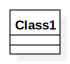
\includegraphics{language/main}
\caption{This is the caption of the figure displaying a white eagle and
a white horse on a snow field}
\end{figure}
